\section{Estensione del modello}
\label{sec:Critica}
Il modello presentato nella \autoref{subsec:DescModello} e utilizzato per gli esempi nella \autoref{sec:Applicazioni} non permette di descrivere adeguatamente un particolare esempio di interesse.
Consideriamo la seguente rete:
\begin{figure}[h!]
\centering

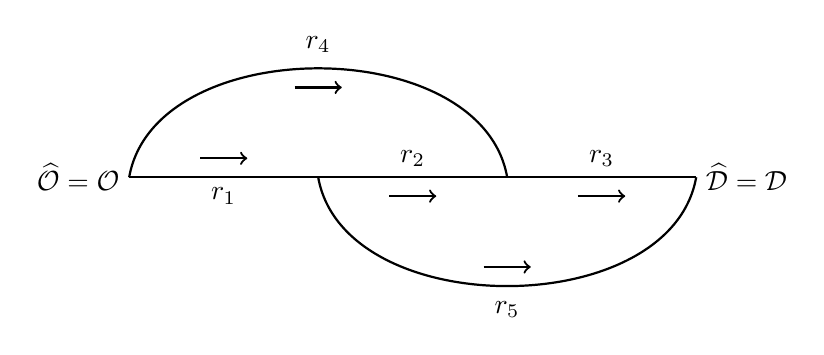
\begin{tikzpicture}[scale=1.2, rotate=-90]

% Nodi principali
\coordinate (A) at (0,0);
\coordinate (B) at (0,6);
\coordinate (Y) at (0,2);
\coordinate (X) at (0,4);

% Segmento principale
\draw[thick] (A) -- (B);

% Arco superiore
\draw[thick]
(B) to[out=-10,in=10] (Y);

% Arco inferiore
\draw[thick]
(A) to[out=170,in=-170] (X);

% Collegamento centrale tratteggiato
\draw[thick, dashed] (Y) -- (X);

% Freccia direzione
\draw[->, thick] (-0.2,0.75) -- (-0.2,1.25);
\draw[->, thick] (0.2,2.75) -- (0.2,3.25);
\draw[->, thick] (0.2,4.75) -- (0.2,5.25);
\draw[->, thick] (-0.95,1.75) -- (-0.95,2.25);
\draw[->, thick] (0.95,3.75) -- (0.95,4.25);

% Etichette
\node[left] at (A) {$\widehat{\mathcal{O}} = \widecheck{\mathcal{O}}$};
\node[right] at (B) {$\widehat{\mathcal{D}} = \widecheck{\mathcal{D}}$};

% Etichette archi
\node at (0.2, 1) {$r_1$};
\node at (-0.2,3) {$r_2$};
\node at (-0.2, 5) {$r_3$};
\node at (-1.4,2) {$r_4$};
\node at (1.4, 4) {$r_5$};

\end{tikzpicture}

\end{figure}

Pensiamo a $(r_1, r_2, r_3)$ come ad una superstrada. In situazioni di traffico moderato ($\widehat{\zeta}$ e $\widecheck{\zeta}$ non troppo elevati) entrambe le popolazioni lo utilizzano per arrivare a destinazione.
Le strade $r_4$ e $r_5$ rappresentano, invece, delle "scorciatoie", convenienti solo in caso di traffico intenso sulla strada principale ($\widehat{\zeta}$ e $\widecheck{\zeta}$ elevati). Il motivo
per cui queste ultime due strade sono opzioni allettanti per i guidatori è la precedenza che essi hanno in uscita da esse: i veicoli provenienti da $r_4$ hanno precedenza sui veicoli
provenienti da $r_2$ (analogo per i veicoli su $r_5$ rispetto a quelli su $r_3$).

Consideriamo apparteneti alla popolazione \textit{hat} i guidatori che conoscono le "scorciatoie" $r_4$ e $r_5$, mentre i guidatori di \textit{check} ne ignorano l'esistenza:

\begin{equation*}
\begin{array}{r @{\hspace{2cm}} r}

\widehat{\gamma}_1 = (r_1, r_2, r_3) &
\widecheck{\gamma}_1 = (r_1, r_2, r_3)\\

\widehat{\gamma}_2 = (r_4, r_3) & \\

\widehat{\gamma}_3 = (r_1, r_5) & \\
$$
\end{array}
\end{equation*}

Realisticamente, in una situazione di traffico intenso, i guidatori \textit{hat} utilizzano le scorciatoie, sfruttando la precedenza
sul percorso principale per evitare il traffico intenso. Tentiamo di descrivere questa situazione con il modello in \autoref{sec:Modello}.

Definiamo dunque le funzioni di costo:
\begin{equation}
\begin{array}{r @{\hspace{2cm}} r}

\widehat{\tau}_1(\eta) = 30+\widehat{\eta}+\widecheck{\eta} &
\widecheck{\tau}_1(\eta) = 30+\widehat{\eta}+\widecheck{\eta} \\

\widehat{\tau}_2(\eta) = 30+\widehat{\eta}+\widecheck{\eta} &
\widecheck{\tau}_2(\eta) = 30+\widehat{\eta}+\widecheck{\eta} \\

\widehat{\tau}_3(\eta) = 5+\widehat{\eta}+\widecheck{\eta} &
\widecheck{\tau}_3(\eta) = 5+\widehat{\eta}+\widecheck{\eta} \\

\widehat{\tau}_4(\eta) = 135+\widehat{\eta} &
\widecheck{\tau}_4(\eta) =  +\infty\\

\widehat{\tau}_5(\eta) = 105+\widehat{\eta} &
\widecheck{\tau}_5(\eta) = +\infty 
$$
\end{array}
\label{eq:13}
\end{equation}
La variazione nel numero di veicoli nelle due popolazioni da $\widehat{\zeta} = \widecheck{\zeta} = 1$ a $\widehat{\zeta} = \widecheck{\zeta} = 101$ comporta (vedi \autoref{script:22}):

\newpage
\vspace*{-4cm}

\begin{figure}[H]
\centering

\begin{tabular}{cc}

\includegraphics[height=6cm]{../figures/Es3/grafico_main_hat_Variazione_del_numero_di_individui_nella_popolazione.png} &

\includegraphics[height=6cm]{../figures/Es3/grafico_main_check_Variazione_del_numero_di_individui_nella_popolazione.png} \\


\includegraphics[height=6cm]{../figures/Es3/grafico_hat/hat_theta_1_Variazione_del_numero_di_individui_nella_popolazione.png} &

\includegraphics[height=6cm]{../figures/Es3/grafico_check/check_theta_1_Variazione_del_numero_di_individui_nella_popolazione.png} \\


\includegraphics[height=6cm]{../figures/Es3/grafico_hat/hat_theta_2_Variazione_del_numero_di_individui_nella_popolazione.png} &
\rule{0pt}{6cm} \\


\includegraphics[height=6cm]{../figures/Es3/grafico_hat/hat_theta_3_Variazione_del_numero_di_individui_nella_popolazione.png} &
\rule{0pt}{6cm} \\

\end{tabular}
\end{figure}

Si ottiene un maggiore aumento del tempo di viaggio per la popolazione \textit{check} rispetto a quello per la popolazione \textit{hat}.
Ciò è dato dal fatto che i guidatori \textit{check} sono costretti a cedere la precedenza, aumentando il tempo di viaggio già elevato a causa della forte presenza di veicoli nella rete. Facendo crescere, dunque, il costo delle
due scorciatoie si dovrebbe ottenere un miglioramento nel tempo di percorrenza della rete per \textit{check}. 

Ponendo $\widehat{\zeta} = \widecheck{\zeta} = 30$ possiamo far variare i costi di $\widehat{\tau}_4$ e $\widehat{\tau}_5$ avendo come situazione iniziale
l'utilizzo delle scorciatoie da parte della popolazione \textit{hat}. Aumentiamo i due costi da $\widehat{\tau}_4(\eta) = 135+\widehat{\eta}$ a $\widehat{\tau}_4(\eta) = 205+\widehat{\eta}$
e da $\widehat{\tau}_5(\eta) = 105+\widehat{\eta}$ a $\widehat{\tau}_5(\eta) = 175+\widehat{\eta}$. Questa operazione restituisce (vedi \autoref{script:23}):

\newpage
\vspace*{-4cm}

\begin{figure}[H]
\centering

\begin{tabular}{cc}

\includegraphics[height=6cm]{../figures/Es3/grafico_main_hat_Variazione_del_costo_delle_strade.png} &

\includegraphics[height=6cm]{../figures/Es3/grafico_main_check_Variazione_del_costo_delle_strade.png} \\


\includegraphics[height=6cm]{../figures/Es3/grafico_hat/hat_theta_1_Variazione_del_costo_delle_strade.png} &

\includegraphics[height=6cm]{../figures/Es3/grafico_check/check_theta_1_Variazione_del_costo_delle_strade.png} \\


\includegraphics[height=6cm]{../figures/Es3/grafico_hat/hat_theta_2_Variazione_del_costo_delle_strade.png} & 
\rule{0pt}{6cm}\\


\includegraphics[height=6cm]{../figures/Es3/grafico_hat/hat_theta_3_Variazione_del_costo_delle_strade.png} &
\rule{0pt}{6cm} \\

\end{tabular}
\end{figure}
Il modello definito in \autoref{sec:Modello} non può tenere conto delle precedenze: i guidatori \textit{hat} smettono progressivamente di utilizzare le scorciatoie
(dato che i costi delle stesse aumentano), ma il tempo di percorrenza della rete per i veicoli \textit{check} non migliora. 

Se vogliamo descrivere meglio il comportamento reale è necessario che il costo di una strada di dipendere anche dalla popolazione presente su un'altra.
Servirebbe dunque far dipendere i tempi di percorrenza che costituiscono il percorso principale non solo dalla concentrazione di veicoli sulla loro relativa strada,
ma anche da $\theta_4$ e $\theta_5$. Questa necessità comporta una generalizzazione del modello, che non intacca altre definizioni, mentre il \autoref{th:1} perde, però, la sua
validità. Modificare leggermente l'enunciato e rifare la dimostrazione è comunque possibile, sembrerebbe anche abbastanza semplicemente. È bene notare in ogni
caso che in questa sezione ci stiamo limitando ad analizzare una singola istanza di un nuovo modello, la quale dà risultati coerenti e significativi. Questo nuovo modello necessiterebbe di una descrizione
generale e completa, con dimostrazioni ed eventuali definizioni diverse da quelle viste nella \autoref{sec:Modello}.
Applichiamo dunque la nuova estensione:

\begin{equation}
\label{eq:12}
\begin{split}
\begin{array}{rccc}
\widehat{\tau}: & [0,1]^N\times[0,1]^N & \to & \mathbb{R}_+^N \cup \{+\infty\}\\
& (\widehat n,\widecheck n) & \mapsto &
\bigl(
\widehat{\tau}_1(\widehat n,\widecheck n),
\dots,
\widehat{\tau}_N(\widehat n,\widecheck n)
\bigr)
\\[1em]
\widecheck{\tau}: & [0,1]^N\times[0,1]^N & \to & \mathbb{R}_+^N \cup \{+\infty\}\\
& (\widehat n,\widecheck n) & \mapsto &
\bigl(
\widecheck{\tau}_1(\widehat n,\widecheck n),
\dots,
\widecheck{\tau}_N(\widehat n,\widecheck n)
\bigr)
\end{array}
\end{split}
\end{equation}

Le equazioni di costo diventano:

\begin{equation}
\label{eq:14}
\begin{array}{r @{\hspace{2cm}} r}

\widehat{\tau}_1(\eta) = 30+\widehat{\eta}_1 + \widecheck{\eta}_1 + \widehat{\eta}_4 + \widehat{\eta}_5 &
\widecheck{\tau}_1(\eta) = 30+\widehat{\eta}_1 + \widecheck{\eta}_1 + \widehat{\eta}_4 + \widehat{\eta}_5\\

\widehat{\tau}_2(\eta) = 30+\widehat{\eta}_2 + \widecheck{\eta}_2 + \widehat{\eta}_4 + \widehat{\eta}_5&
\widecheck{\tau}_2(\eta) = 30+\widehat{\eta}_2 + \widecheck{\eta}_2 + + \widehat{\eta}_4 + \widehat{\eta}_5 \\

\widehat{\tau}_3(\eta) = 5+\widehat{\eta}_3+\widecheck{\eta}_3 + \widehat{\eta}_5&
\widecheck{\tau}_3(\eta) = 5+\widehat{\eta}_3+\widecheck{\eta}_3 + \widehat{\eta}_5\\

\widehat{\tau}_4(\eta) = 135+\widehat{\eta}_4 &
\widecheck{\tau}_4(\eta) =  +\infty\\

\widehat{\tau}_5(\eta) = 105+\widehat{\eta}_5 &
\widecheck{\tau}_5(\eta) = +\infty 
$$
\end{array}
\end{equation}

Se facciamo nuovamente variare il numero di veicoli da $\widehat{\zeta} = \widecheck{\zeta} = 1$ a $\widehat{\zeta} = \widecheck{\zeta} = 101$ (vedi \autoref{script:24}) e
lo confrontiamo con il risultato ottenuto con i costi definiti in (\autoref{eq:13}):

\newpage
\vspace*{-4cm}
\begin{figure}[H]
\centering
\begin{tabular}{cc}

\includegraphics[height=6cm]{../figures/Es3/grafico_main_hat_Variazione_del_numero_di_individui_nella_popolazione.png} &

\includegraphics[height=6cm]{../figures/Es4/grafico_main_hat_Variazione_del_numero_di_individui_nella_popolazione.png} \\
\end{tabular}
\caption*{Tempo di viaggio \textit{hat} al variare delle popolazioni, a sinistra utilizzando le funzioni di costo definite in (\autoref{eq:13}), a destra utilizzando le funzioni di costo definite in (\autoref{eq:14})}
\end{figure}

\begin{figure}[H]
\centering
\begin{tabular}{cc}

\includegraphics[height=6cm]{../figures/Es3/grafico_main_check_Variazione_del_numero_di_individui_nella_popolazione.png} &

\includegraphics[height=6cm]{../figures/Es4/grafico_main_check_Variazione_del_numero_di_individui_nella_popolazione.png} \\
\end{tabular}
\caption*{Tempo di viaggio \textit{check} al variare delle popolazioni, a sinistra utilizzando le funzioni di costo definite in (\autoref{eq:13}), a destra utilizzando le funzioni di costo definite in (\autoref{eq:14})}
\end{figure}

\begin{figure}[H]
\centering
\begin{tabular}{cc}

\includegraphics[height=6cm]{../figures/Es3/grafico_hat/hat_theta_1_Variazione_del_numero_di_individui_nella_popolazione.png} &

\includegraphics[height=6cm]{../figures/Es4/grafico_hat/hat_theta_1_Variazione_del_numero_di_individui_nella_popolazione.png} \\


\includegraphics[height=6cm]{../figures/Es3/grafico_hat/hat_theta_2_Variazione_del_numero_di_individui_nella_popolazione.png} &

\includegraphics[height=6cm]{../figures/Es4/grafico_hat/hat_theta_2_Variazione_del_numero_di_individui_nella_popolazione.png} \\


\includegraphics[height=6cm]{../figures/Es3/grafico_hat/hat_theta_3_Variazione_del_numero_di_individui_nella_popolazione.png} &

\includegraphics[height=6cm]{../figures/Es4/grafico_hat/hat_theta_3_Variazione_del_numero_di_individui_nella_popolazione.png} \\

\end{tabular}
\caption*{Equilibrio di Nash \textit{hat} al variare delle popolazioni, a sinistra utilizzando le funzioni di costo definite in (\autoref{eq:13}), a destra utilizzando le funzioni di costo definite in (\autoref{eq:14}). Viene tralasciato l'Equilibrio di Nash di \textit{check} in quanto sempre costante}
\end{figure}

Il risultato ottenuto descrive un comportamento simile a quello visto in precedenza. La differenza più evidente è nei valori che assumono le curve dei tempi
di destra: sono maggiori rispetto a quelli di sinistra. Ovviamente ciò è causato dalla modifica ai tempi delle strade nel percorso principale, che dipendono anche dal numero di auto sulle
scorciatoie.

Controlliamo ora l'effetto dell'aumento dei costi da $\widehat{\tau}_4(\eta) = 135+\widehat{\eta}$ a $\widehat{\tau}_4(\eta) = 205+\widehat{\eta}$
e da $\widehat{\tau}_5(\eta) = 105+\widehat{\eta}$ a $\widehat{\tau}_5(\eta) = 175+\widehat{\eta}$ con $\widehat{\zeta} = \widecheck{\zeta} = 30$ (vedi \autoref{script:24}). Confrontiamo il risultato ottenuto
con quello ricavato in precedenza applicando la stessa variazione ai costi definiti nell'(\autoref{eq:13}). Tralasciamo il grafico rappresentante 
l'equilibrio di Nash della popolazione \textit{check}, data la presenza di un unico percorso per essa:

\newpage

\begin{figure}[H]
\centering
\begin{tabular}{cc}

\includegraphics[height=6cm]{../figures/Es3/grafico_main_hat_Variazione_del_costo_delle_strade.png}&

\includegraphics[height=6cm]{../figures/Es4/grafico_main_hat_Variazione_del_costo_delle_strade.png}\\
\end{tabular}
\caption*{Tempo di viaggio \textit{hat} al variare del costo delle scorciatoie, a sinistra utilizzando le funzioni di costo definite in (\autoref{eq:13}), a destra utilizzando le funzioni di costo definite in (\autoref{eq:14})}
\end{figure}

\begin{figure}[H]
\centering
\begin{tabular}{cc}

\includegraphics[height=6cm]{../figures/Es3/grafico_main_check_Variazione_del_costo_delle_strade.png} &

\includegraphics[height=6cm]{../figures/Es4/grafico_main_check_Variazione_del_costo_delle_strade.png} \\
\end{tabular}
\caption*{Tempo di viaggio \textit{check} al variare del costo delle scorciatoie, a sinistra utilizzando le funzioni di costo definite in (\autoref{eq:13}), a destra utilizzando le funzioni di costo definite in (\autoref{eq:14})}
\end{figure}

\begin{figure}[H]
\centering

\begin{tabular}{cc}


\includegraphics[height=6cm]{../figures/Es3/grafico_hat/hat_theta_1_Variazione_del_costo_delle_strade.png} &

\includegraphics[height=6cm]{../figures/Es4/grafico_hat/hat_theta_1_Variazione_del_costo_delle_strade.png} \\


\includegraphics[height=6cm]{../figures/Es3/grafico_hat/hat_theta_2_Variazione_del_costo_delle_strade.png} &

\includegraphics[height=6cm]{../figures/Es4/grafico_hat/hat_theta_2_Variazione_del_costo_delle_strade.png} \\


\includegraphics[height=6cm]{../figures/Es3/grafico_hat/hat_theta_3_Variazione_del_costo_delle_strade.png} &

\includegraphics[height=6cm]{../figures/Es4/grafico_hat/hat_theta_3_Variazione_del_costo_delle_strade.png} \\
\end{tabular}
\caption*{A sinistra la variazione dell'Equilibrio di Nash calcolato utilizzando le funzioni di costo definite in (\autoref{eq:13}). A destra la variazione dell'Equilibrio di Nash calcolato utilizzando le funzioni di costo definite in (\autoref{eq:14}).}
\end{figure}

I costi definiti nell'(\autoref{eq:14}) permettono di rappresentare il comportamento atteso in modo più accurato: se i guidatori \textit{hat} smettono
di utilizzare le scorciatoie il tempo di viaggio della popolazione \textit{check} diminuisce, dato che non devono più cedere la precedenza ai veicoli che
provengono da $r_4$ ed $r_5$.